\section{Experiments and Results}
\label{sec:Expt}
As presented in the model in Section~\ref{sec:ProbForm} we have a complete optimization
model with several integer variables for foreground-background labels.

%We will test the performance of our solution on the 
%Berkeley Motion Segmentation Dataset as provided by %\cite{brox2010object}.
%The dataset has 26 video sequences with pixel-accurate segmentation %annotation of moving objects. A total of 189 frames are annotated.
%
%We will evaluate results from our approach and compare the performance %with that of \cite{Felzenszwalb2010b}, \cite{Komodakis2011a}
%and \cite{brox2010object} on this dataset.
%
%Furthermore multiple decoupling strategies will implementation and %compared,
%like decoupling time frames v/s decoupling in space. Finally a dual %decomposition
%method with also be explored and compared qualitatively with %\cite{Komodakis2007a}.

%We plan on completing the implementation in MATLAB with the use of CVX %and CPLEX
%optimization libraries.

We synthetically generate videos which have a foreground object that undergoes translations, rotations and shrinkage. We use this synthetic data to fine-tune parameters as well as test the performance of our algorithm. Since the ground-truth segmentations of the synthetic data are known, the performance of the algorithm on the data can be readily measured. Unfortunately, due to the complexity issues mentioned above, we are unable to test our approach on real video datsets as the computational time requirement is currently not feasible. We see in Figure \ref{fig:trackSquare} that our algorithm perfectly handles simple cases of tracking synthetic objects with random motions.

\begin{figure*}[h]
\begin{center}
	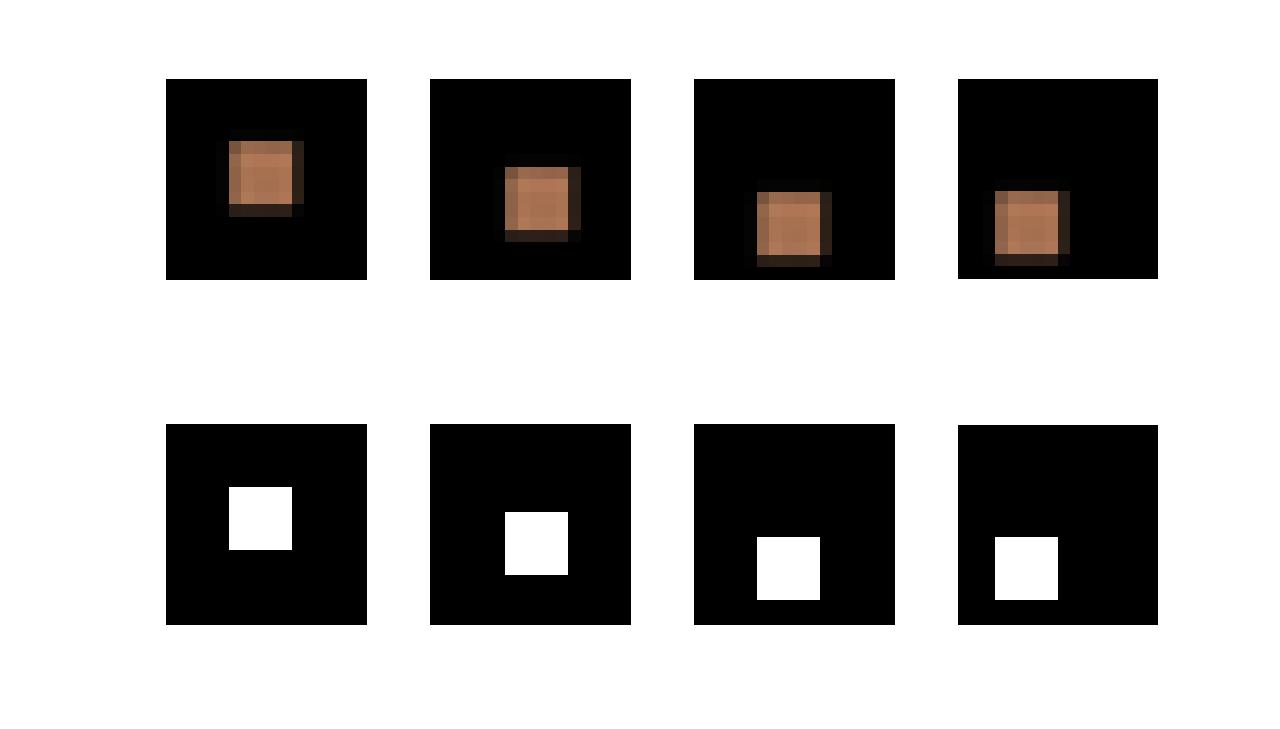
\includegraphics[scale=0.35]{figures/easy_square_tracking.jpg}
	\caption{Results of tracking a simple synthetic object. White pixels represent inferred foreground segmentation mask}
	\label{fig:trackSquare}
\end{center}
\end{figure*}

\begin{figure*}[h]
\begin{center}
	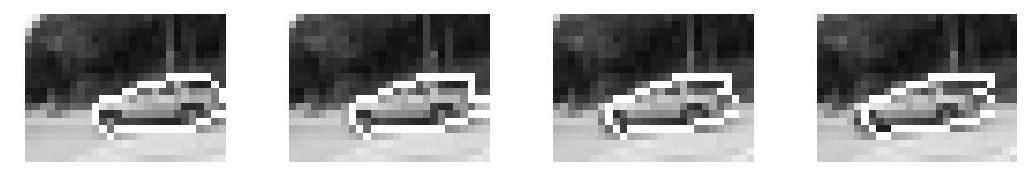
\includegraphics[scale=0.35]{figures/car_tracking.jpg}
	\caption{Results of tracking a downsampled real video without using first order approximations. White pixels represent inferred foreground segmentation boundary}
	\label{fig:trackCar}
\end{center}
\end{figure*}

\begin{figure*}[h]
\begin{center}
	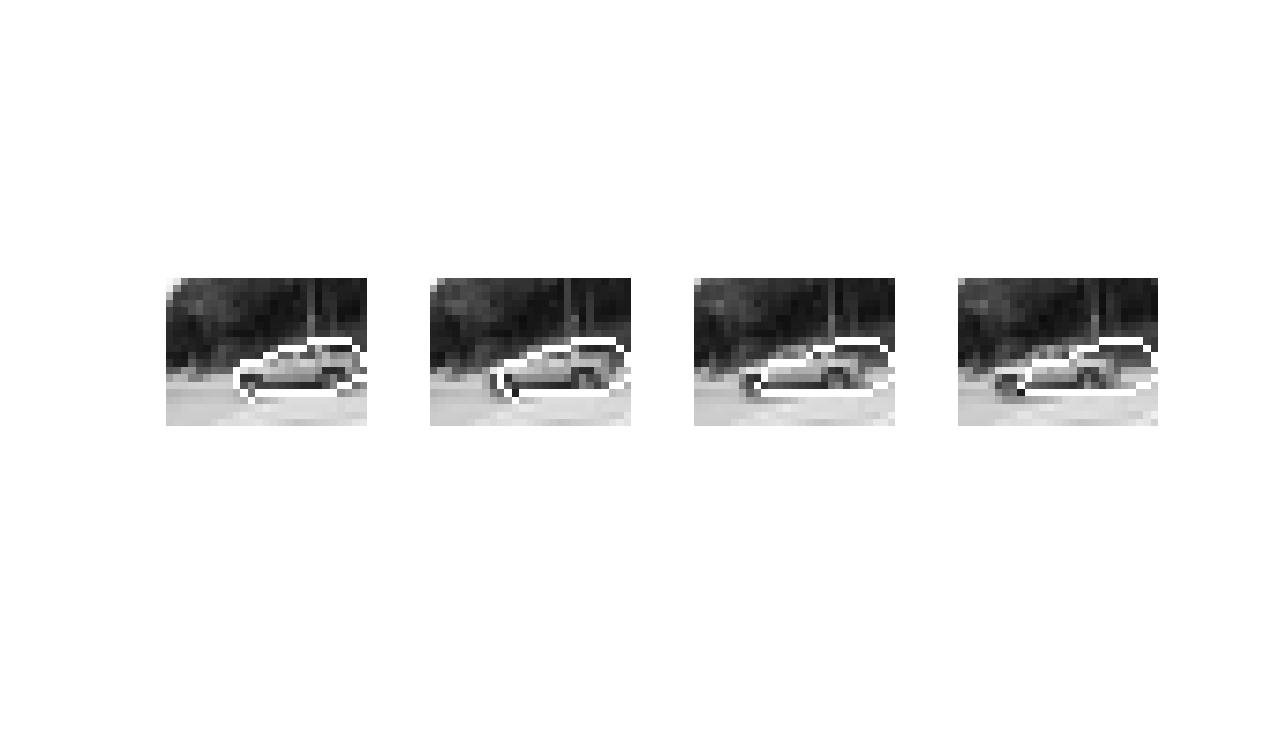
\includegraphics[scale=0.35]{figures/horn_schunk_car_tracking.jpg}
	\caption{Results of tracking a downsampled real video using first-order approximations in reformulation. White pixels represent inferred foreground segmentation boundary}
	\label{fig:HStrackCar}
\end{center}
\end{figure*}

In Figures ~\ref{fig:trackCar} and ~\ref{fig:HStrackCar}, we compare the performance of our two formulations on a highly down-sampled real video. We see that the algorithm without the first order approximations performs reasonably well as opposed to the faster version which uses the first order approximations we define in our reformulation.